\documentclass[hyperref=colorlinks]{beamer}
\mode<presentation>
\usetheme{iclpt}
\setbeamertemplate{navigation symbols}{}
\setbeamertemplate{headline}{
\begin{beamercolorbox}[leftskip=.2cm,rightskip=.2cm,topskip=.2cm,ht=1.1cm,dp=0.1cm,wd=\textwidth]{institute in head/foot}
  
\includegraphics[height=1cm]{icl.pdf}
  \hfill
  
\includegraphics[height=1cm]{../Pics/CMS-Color.pdf}
\end{beamercolorbox}
}
\setbeamertemplate{footline}{
\begin{beamercolorbox}[ht=.55cm,dp=0.4cm,wd=\textwidth,leftskip=.3cm]{author in head/foot}%
  \begin{minipage}[c]{5cm}%
    \usebeamerfont{author in head/foot}
    \insertshortauthor 
    \insertshorttitle
    \end{minipage}\hfill%
  \insertframenumber{} / \pageref{lastframe}
  \hfill
  \begin{minipage}{6cm}
    \hfill
  \end{minipage}
\end{beamercolorbox}%
}

\usepackage{color}
\usepackage{tabularx,colortbl}
\usepackage{graphicx}
\usepackage{pdfpages}
\usepackage{feynmp}
\usepackage{multirow}
\DeclareGraphicsRule{*}{mps}{*}{}

\title{\vspace{-0.2cm} VBF Higgs to Invisible Trigger Efficiencies}
%\subtitle{This result: HIG-15-012 \\ Contributing analyses: HIG-13-030, HIG-14-038, EXO-12-055}
\author[P. Dunne]{\underline{P. Dunne}}
\titlegraphic{
  \vspace{-0.7cm}
  %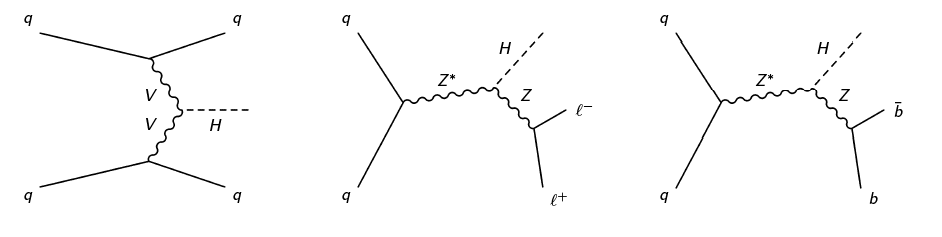
\includegraphics[width=\textwidth]{TalkPics/invcomb021213/feyndiags}
%% \begin{fmfgraph*}(100,70)
%%         \fmfleft{i1,i2}
%%         \fmfright{o1,o2,o3}
%%         \fmf{fermion}{i1,v1,o1}
%%         \fmf{fermion}{i2,v2,o3}
%%         \fmf{phantom,tension=4/5}{v1,v2}
%%         \fmffreeze
%%         \fmf{photon,label=$W,,Z$}{v1,v3}
%%         \fmf{photon,label=$W,,Z$}{v2,v3}
%%         \fmf{dashes}{v3,o2}
%%         \fmflabel{$q$}{i1}
%%         \fmflabel{$q$}{i2}
%%         \fmflabel{$q$}{o1}
%%         \fmflabel{$q$}{o3}
%%         \fmflabel{$H$}{o2}
%%       \end{fmfgraph*}
}
\date{}
\begin{document}
\begin{fmffile}{hexotrig261015feyndiags}

%TITLE PAGE
\section{Title}
\begin{frame}
  \titlepage
  
\end{frame}

%!!CLOSURE TEST STATEMENT PU jet ID
%OUTLINE
\begin{frame}
  \frametitle{Reminder}
  \scriptsize
  \begin{block}{}
    \begin{itemize}
      \item Slow trigger turn on seen in met (300 GeV 95\% efficiency) and jet 2 pt (80 GeV 95\% efficiency
      \item Possible culprits:
      \item[-] Calo prefilter + wrong JEC at HLT
      \item[-] L1 MET turn on
      \item Will investigate L1 MET turn on further in today's slides
      \item Also add HLT\_IsoMu20 to preselection to rule out bias from triggers in SingleMuon
    \end{itemize}
  \end{block}
\end{frame}

\begin{frame}
  \frametitle{L1ETM60 Efficiency: Inclusive}
  \scriptsize
  \begin{block}{}
    \begin{itemize}
    \item Measure L1 ETM turn on
    \item Trigger: L1ETM60
    \item Denominator: SingleMuon events passing HLT\_IsoMu20
    \item 95\% efficient by 200 GeV
    \end{itemize}
  \end{block}
  \centering
  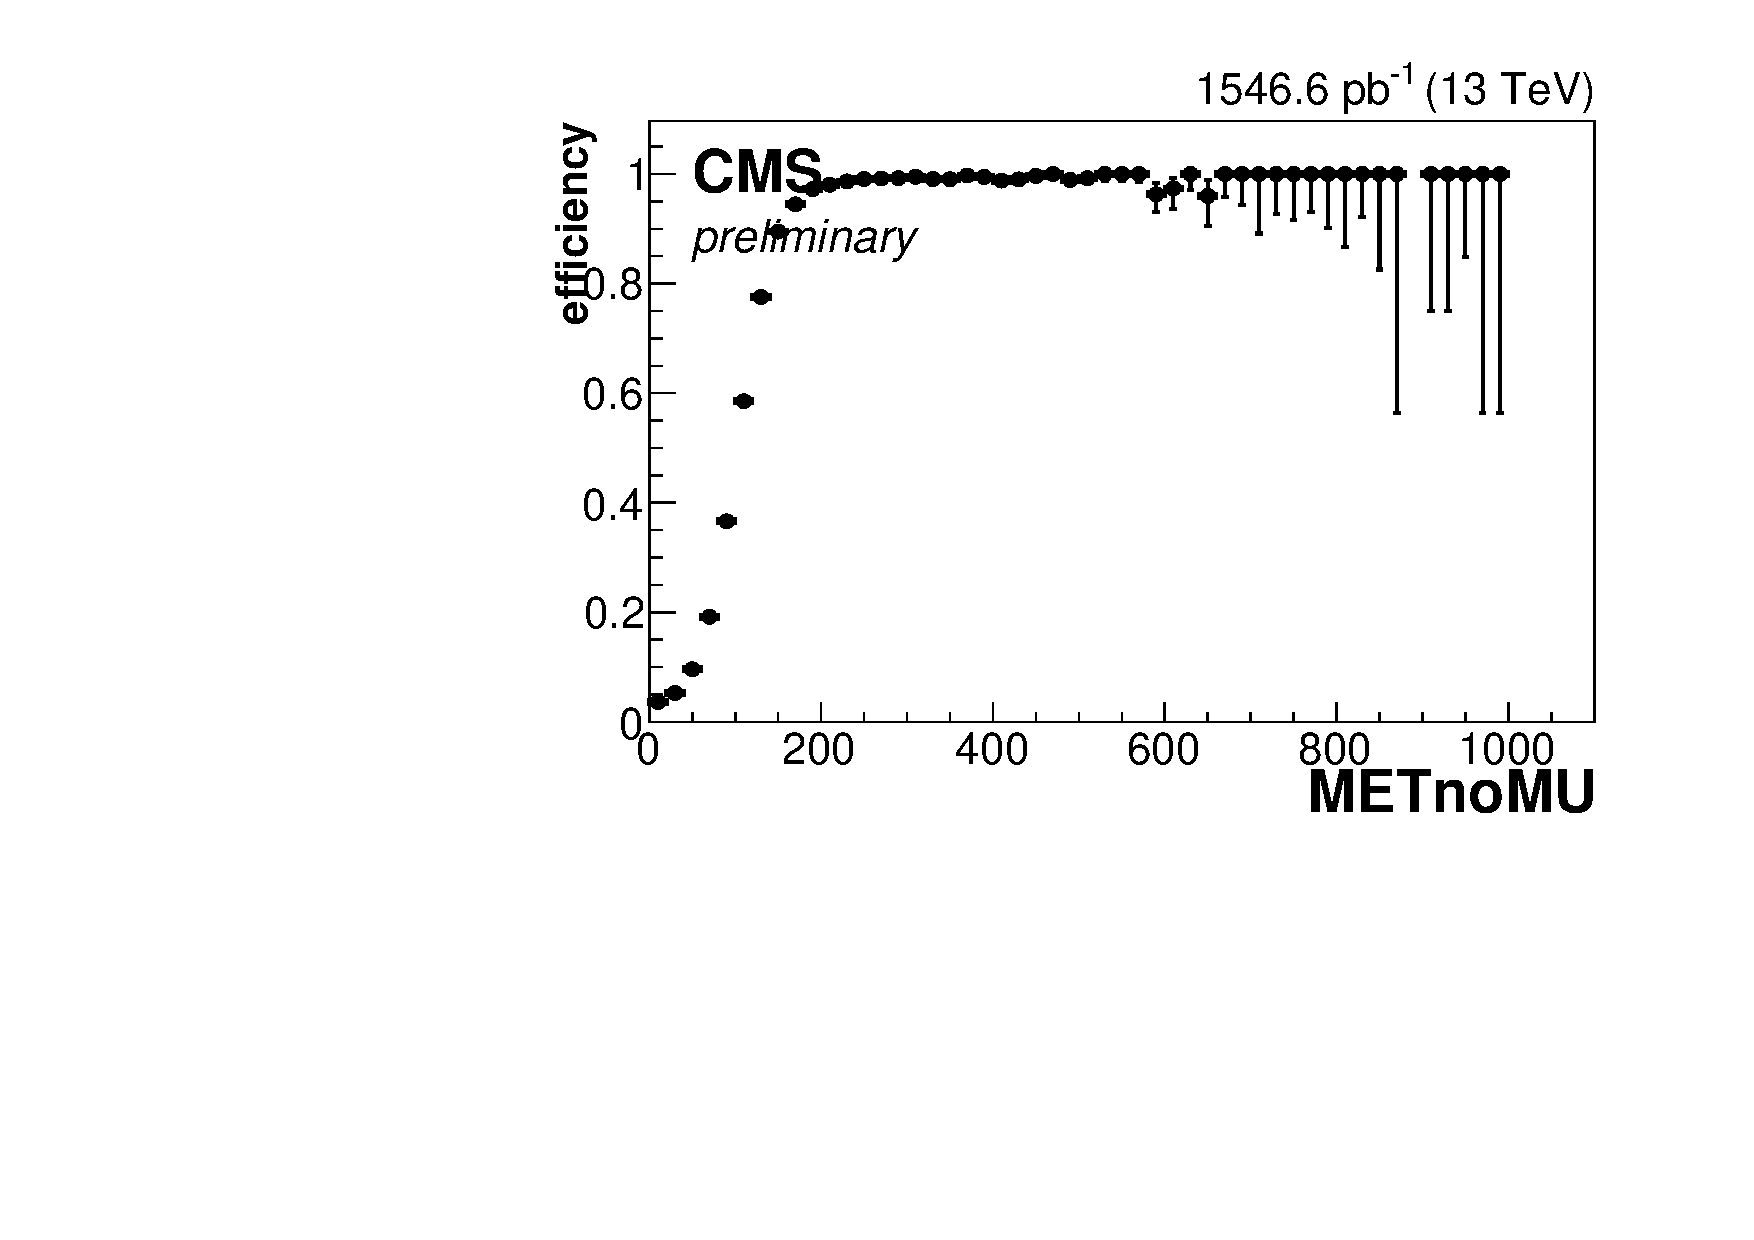
\includegraphics[width=.5\textwidth]{TalkPics/trigeff161115/output_2015Dtrigeff_301015json_l1met60_nocuts_161115/nunu_metnomuons.pdf}
\end{frame}

\begin{frame}
  \frametitle{L1ETM60 Efficiency: VBF phase space}
  \scriptsize
  \begin{block}{}
    \begin{itemize}
    \item Measure L1 ETM turn on when there is a VBF-like dijet
    \item Trigger: L1ETM60
    \item Denominator: SingleMuon events passing HLT\_IsoMu20 and dijet $p_{T}>80$, $M_{jj}>600$, $\Delta\eta_{jj}>3.6$
    \item Good turn on to 150 GeV then shelf
    \end{itemize}
  \end{block}
  \centering
  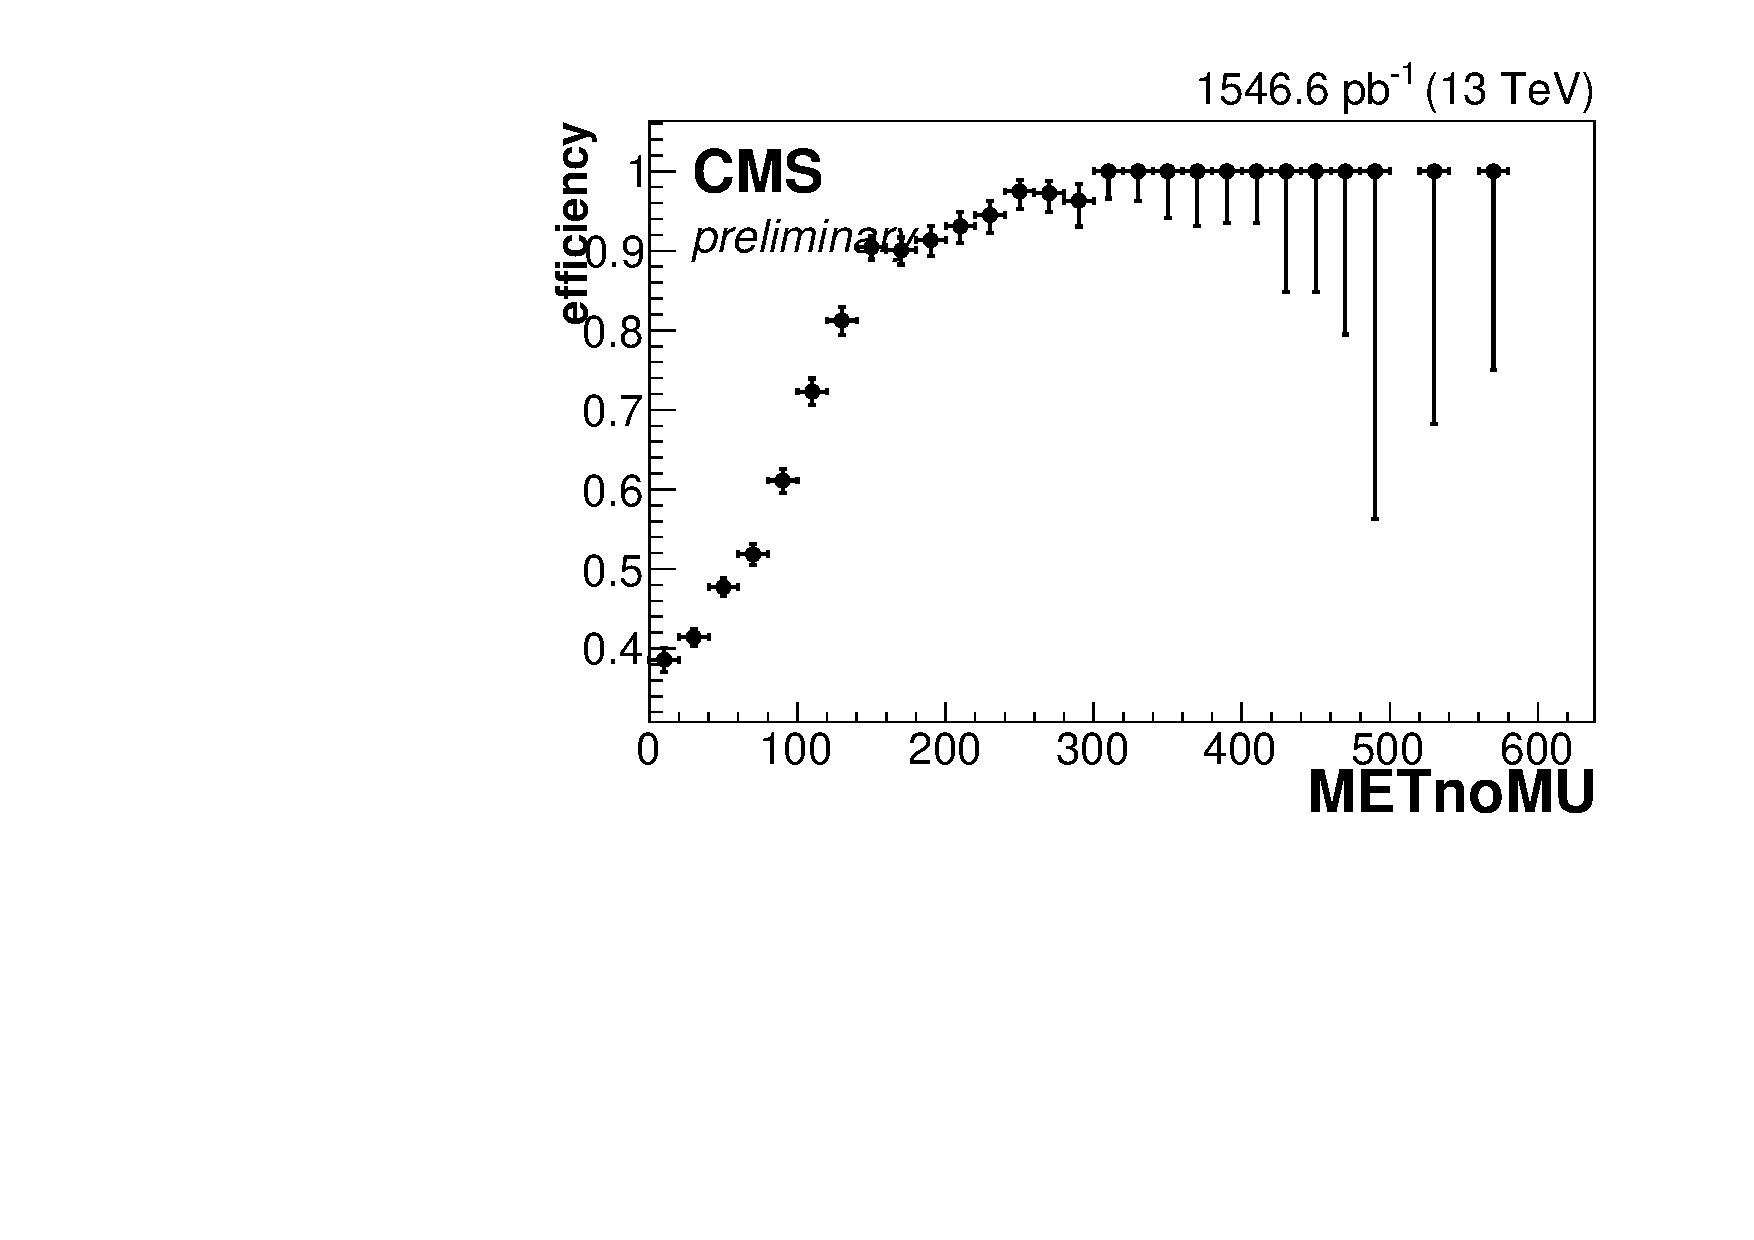
\includegraphics[width=.5\textwidth]{TalkPics/trigeff161115/nunu_metnomuons.pdf}
\end{frame}

\begin{frame}
  \frametitle{L1ETM60 Efficiency: VBF phase space}
  \scriptsize
  \begin{block}{}
    \begin{itemize}
    \item L1 MET only sums up to $|\eta|=$3, shelf seen on previous slide could be due to jets in the HF
    \item Add requirement that both jets have $|\eta|<3$ to the denominator
    \item Good turn on recovered
    \end{itemize}
  \end{block}
  \centering
  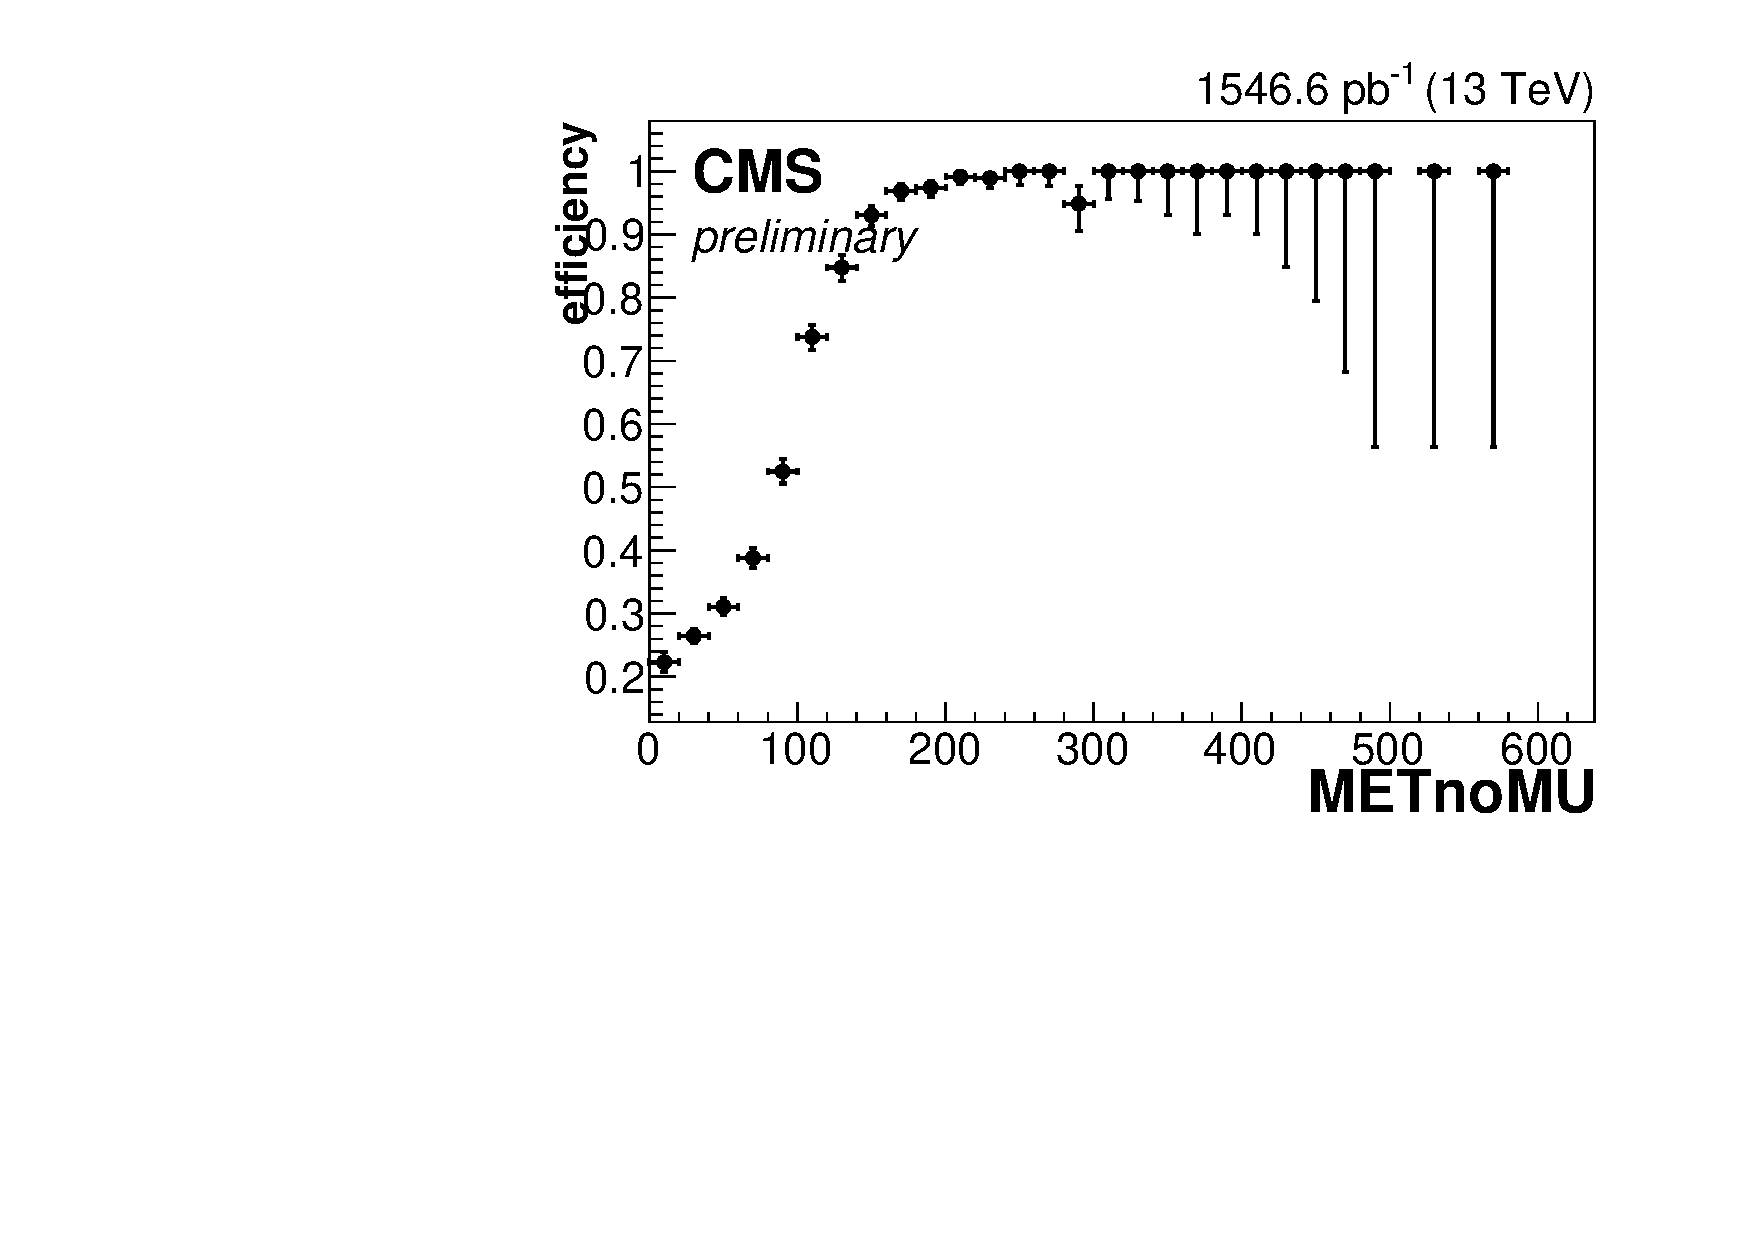
\includegraphics[width=.5\textwidth]{TalkPics/trigeff161115/nunu_metnomuons_bothcentral.pdf}
\end{frame}



\begin{frame}
  \frametitle{Signal trigger efficiency: MET}
  \scriptsize
  \begin{block}{}
    \begin{itemize}
    \item Measure signal trigger efficiency before (right) and after (left) requiring L1ETM60
    \item Trigger: HLT\_DiPFJet40\_DEta3p5\_MJJ600\_PFMETNoMu140
    \item Denominator: SingleMuon events with dijet $p_{T}>80$, $M_{jj}>600$, $\Delta\eta_{jj}>3.6$ plus for left plot only HLT\_IsoMu20 and L1ETM60
    \item Clearly better after L1ETM60 cut: 95\% efficient by 250 GeV
    \end{itemize}
  \end{block}
  \centering
  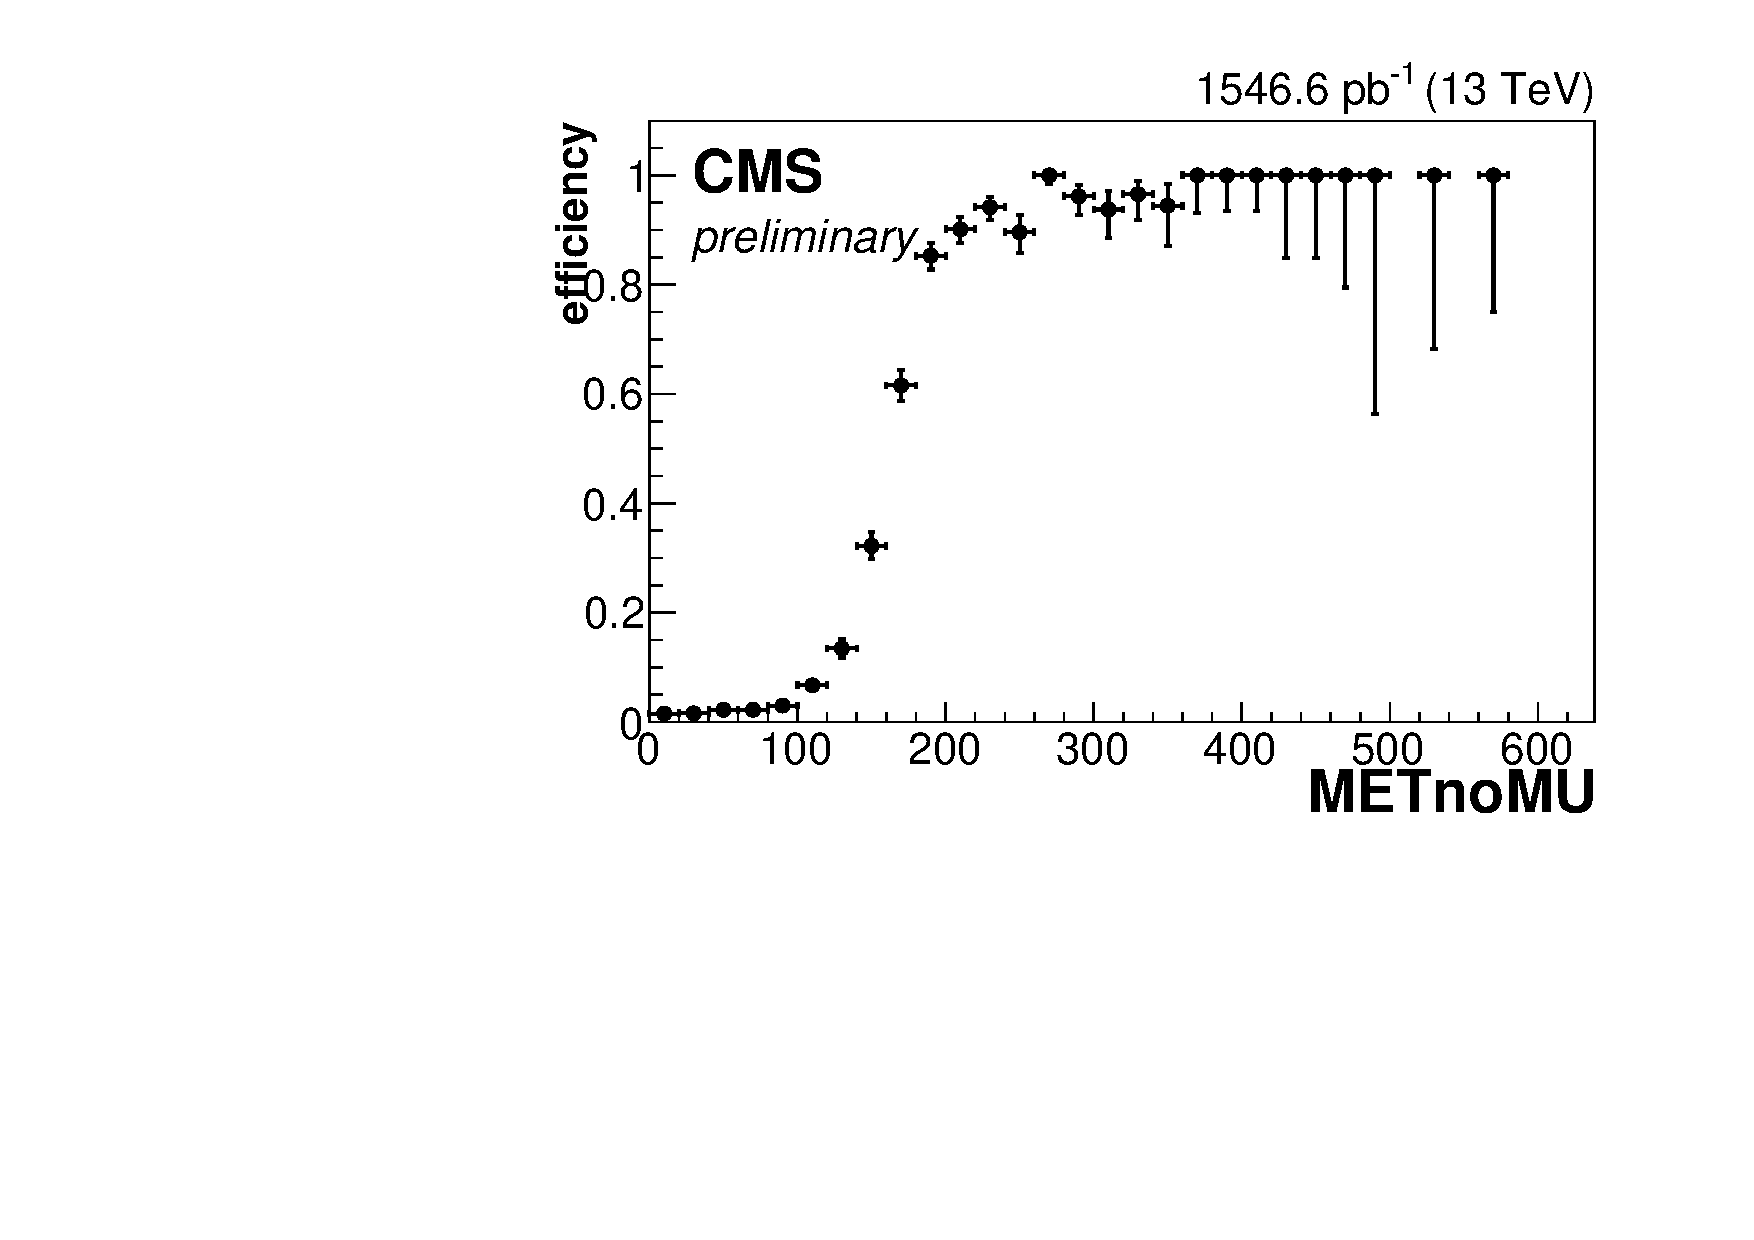
\includegraphics[width=.5\textwidth]{TalkPics/trigeff161115/output_2015Dtrigeff_301015json_sigtrig_l1met60met300jpt80cut_161115/nunu_metnomuons.pdf}
  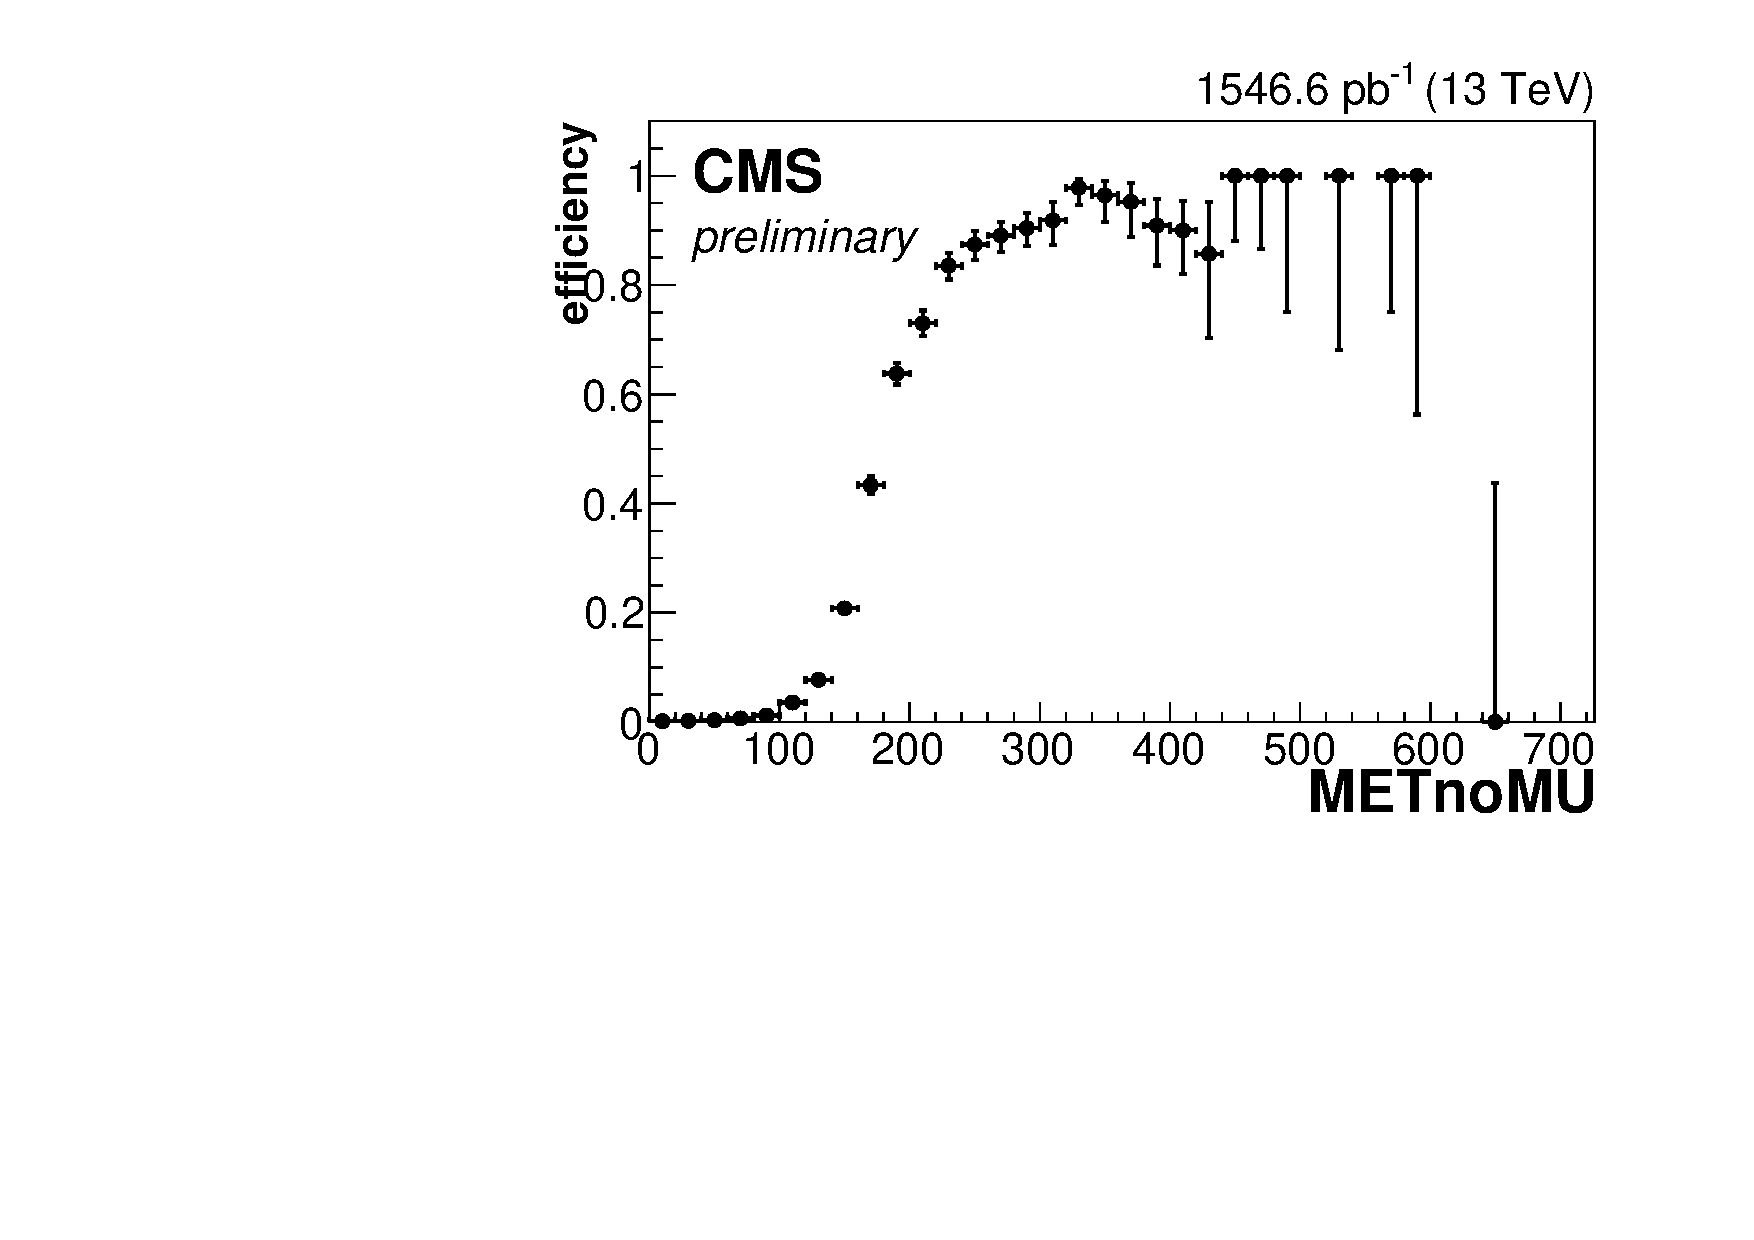
\includegraphics[width=.5\textwidth]{TalkPics/trigeffandpheno041115/nunu_metnomuons.pdf}
\end{frame}

\begin{frame}
  \frametitle{Signal trigger efficiency: jet pt}
  \scriptsize
  \begin{block}{}
    \begin{itemize}
    \item Measure signal trigger efficiency before (right) and after (left) requiring L1ETM60
    \item Trigger: HLT\_DiPFJet40\_DEta3p5\_MJJ600\_PFMETNoMu140
    \item Denominator: SingleMuon events with dijet $METnoMU>300$, $M_{jj}>600$, $\Delta\eta_{jj}>3.6$ plus for left plot only HLT\_IsoMu20 and L1ETM60
    \item Slightly better after L1ETM60 cut: 95\% efficient by 70 GeV
    \end{itemize}
  \end{block}
  \centering
  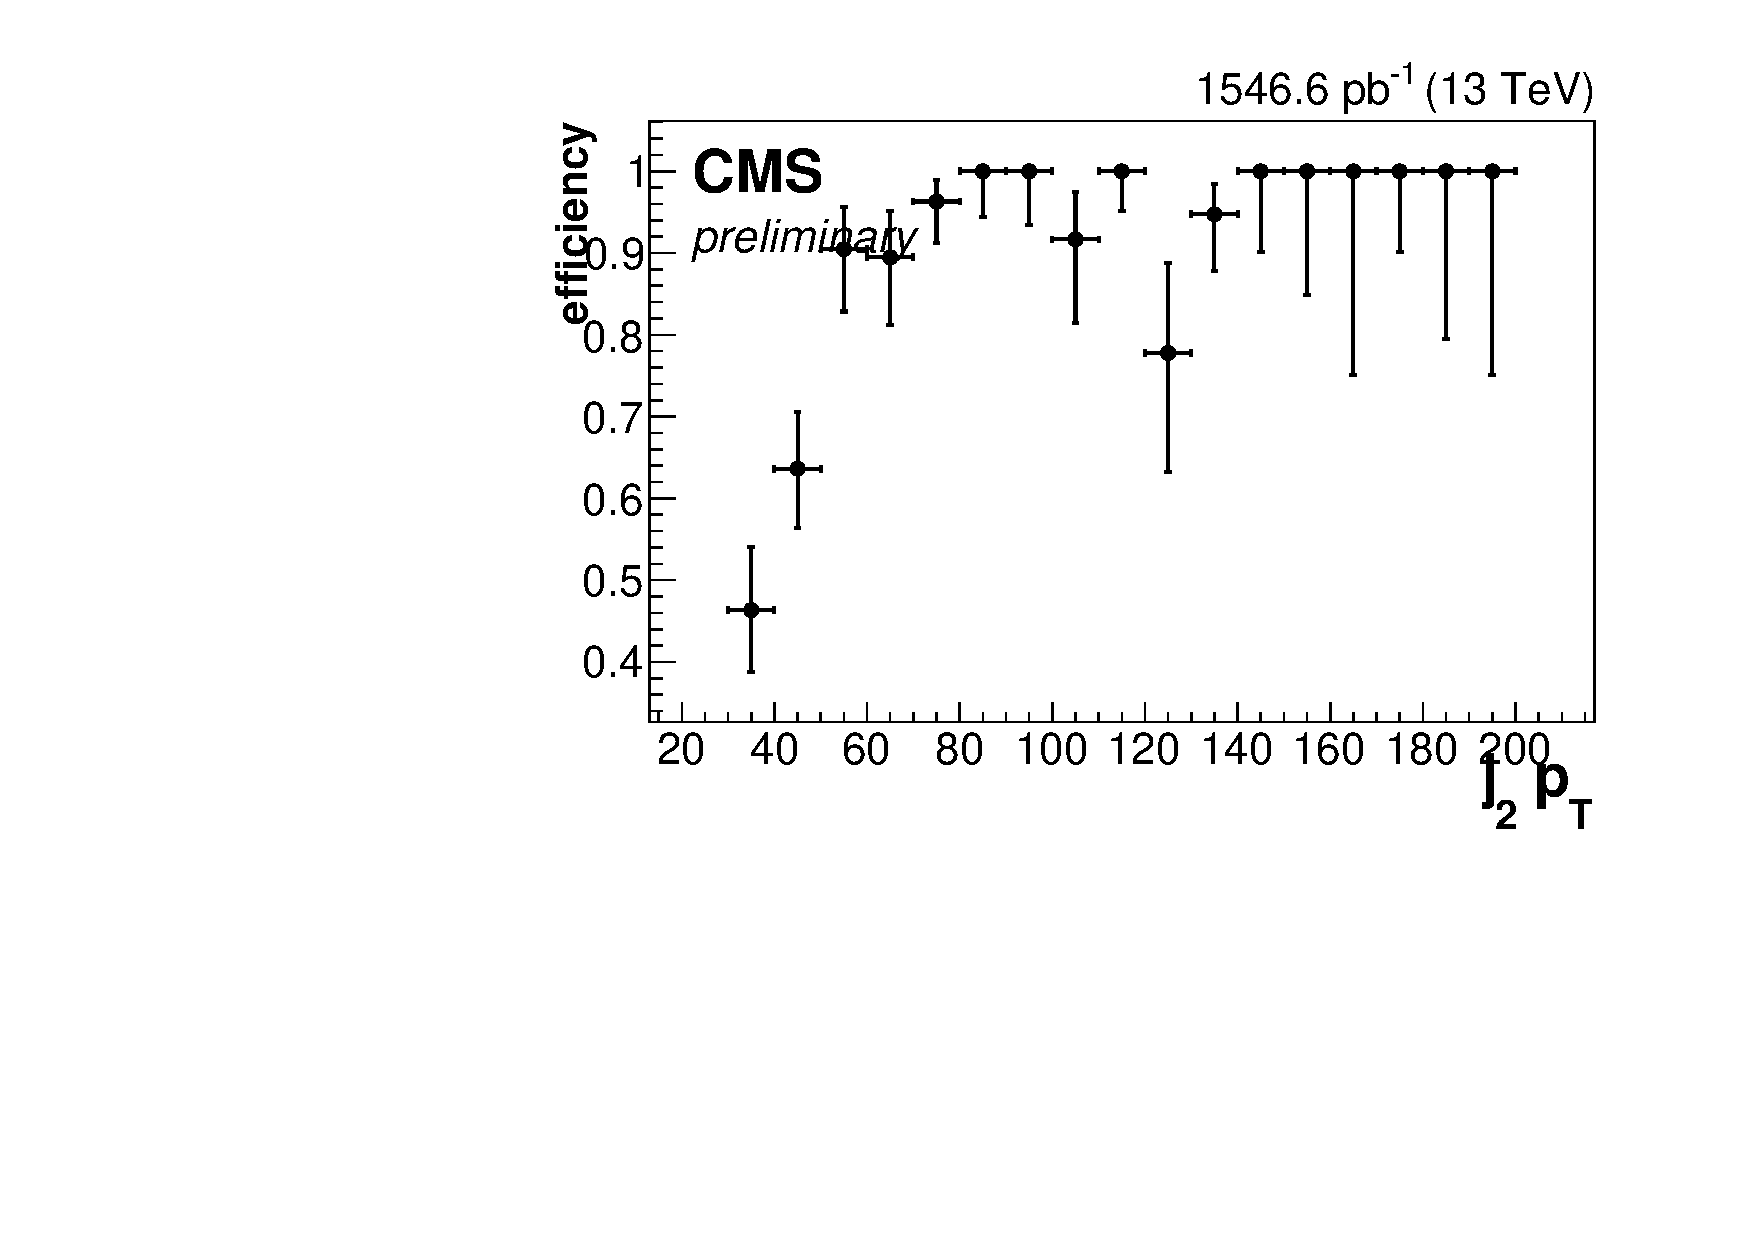
\includegraphics[width=.5\textwidth]{TalkPics/trigeff161115/output_2015Dtrigeff_301015json_sigtrig_l1met60met300jpt80cut_161115/nunu_jet2_pt.pdf}
  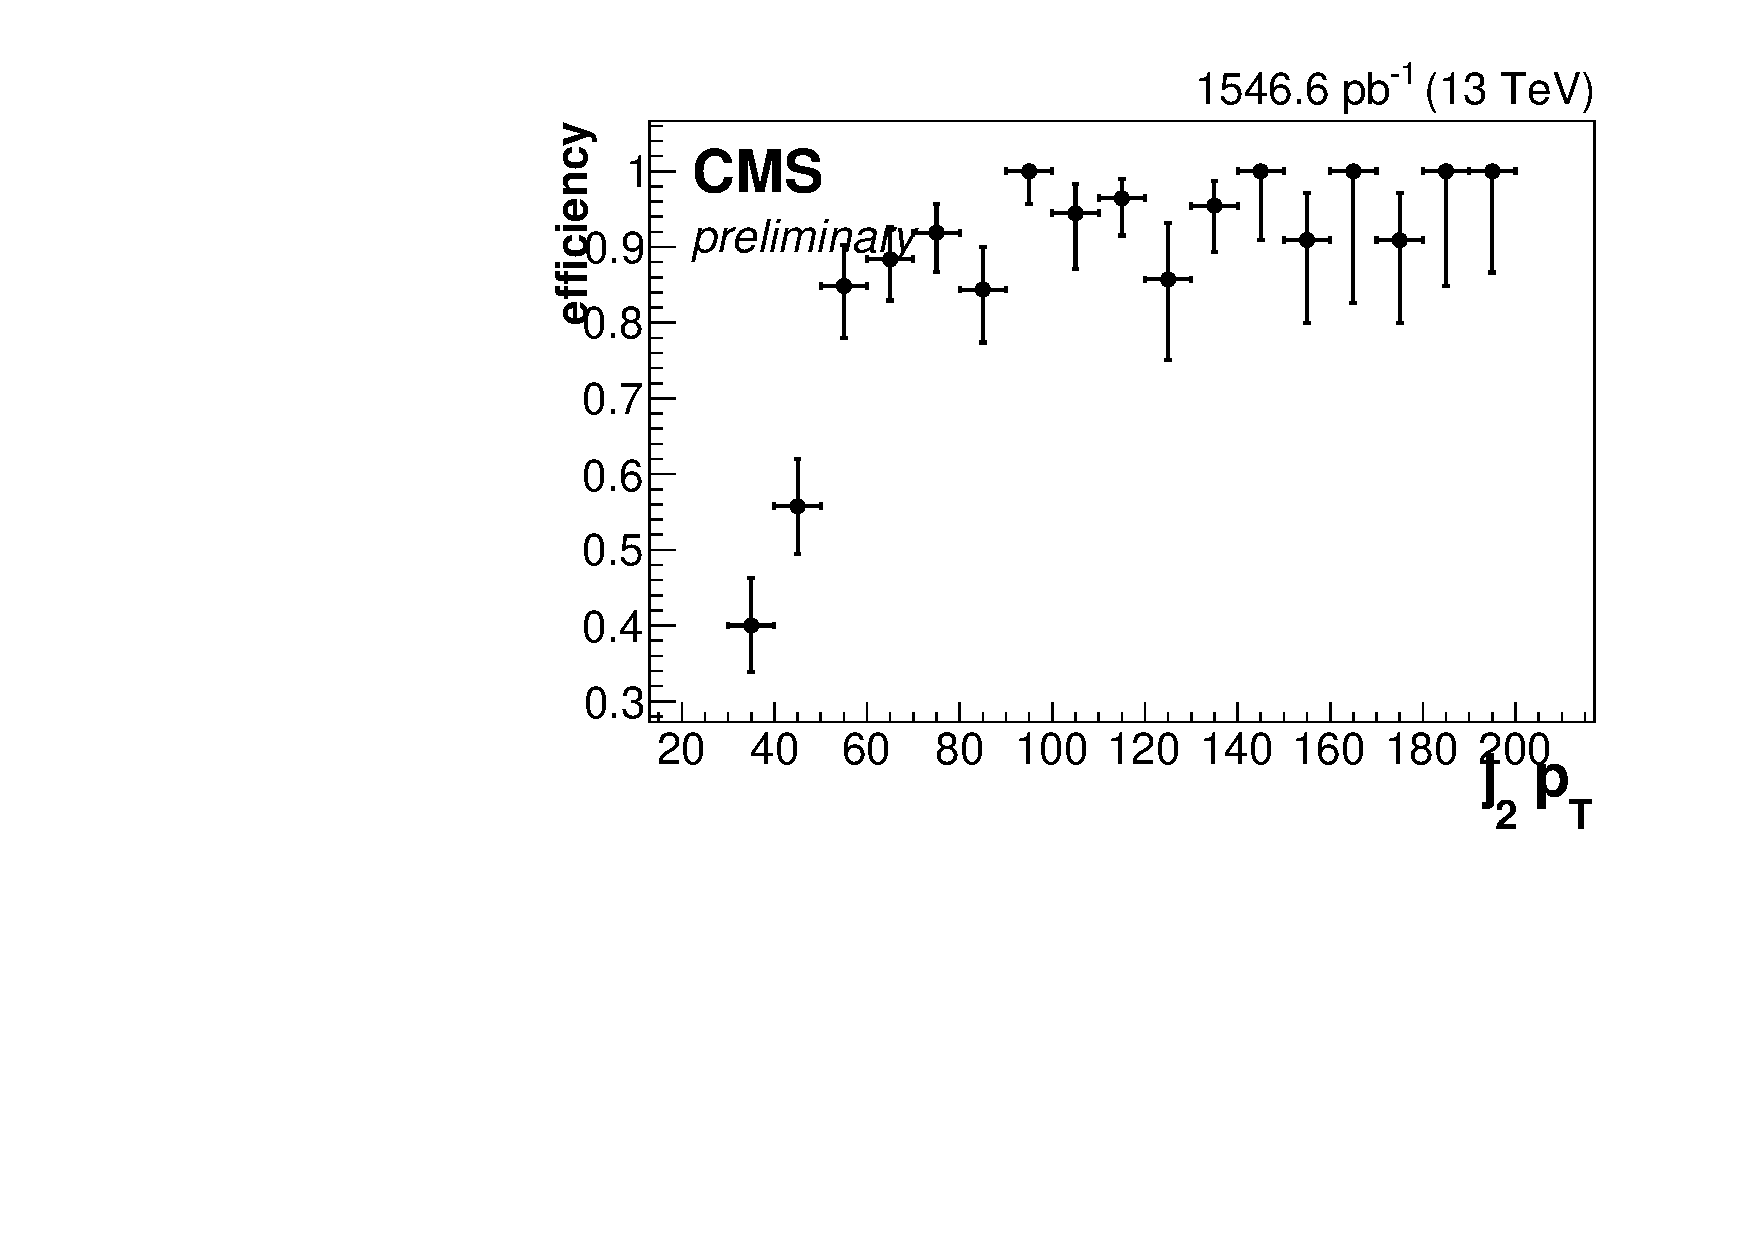
\includegraphics[width=.5\textwidth]{TalkPics/trigeffandpheno041115/nunu_jet2_pt.pdf}
\end{frame}

\begin{frame}
  \frametitle{Calo jet prefilter}
  \scriptsize
  \begin{columns}
    \column{1.1\textwidth}
  \begin{block}{}
    \begin{itemize}
    \item Jet $p_{T}$ still less efficient than run 1: 95\% efficient at 70 GeV compared to 50 GeV
    \item According to \href{https://indico.cern.ch/event/456813/contribution/0/attachments/1178012/1704076/15-10-28_News_PPD.pdf}{this} wrong JEC was used in HLT during Run2015
    \item[-] We have a calo prefilter at 30 GeV
    \item[-] Calo JEC are large so differences could cause the remaining jet pt issues
    \item Plot offline jet pt (x) against trigger calo jet pt (y)
    \item Large differences seen between calo jet pt and offline pt
    \end{itemize}
  \end{block}
  \end{columns}
  \centering
  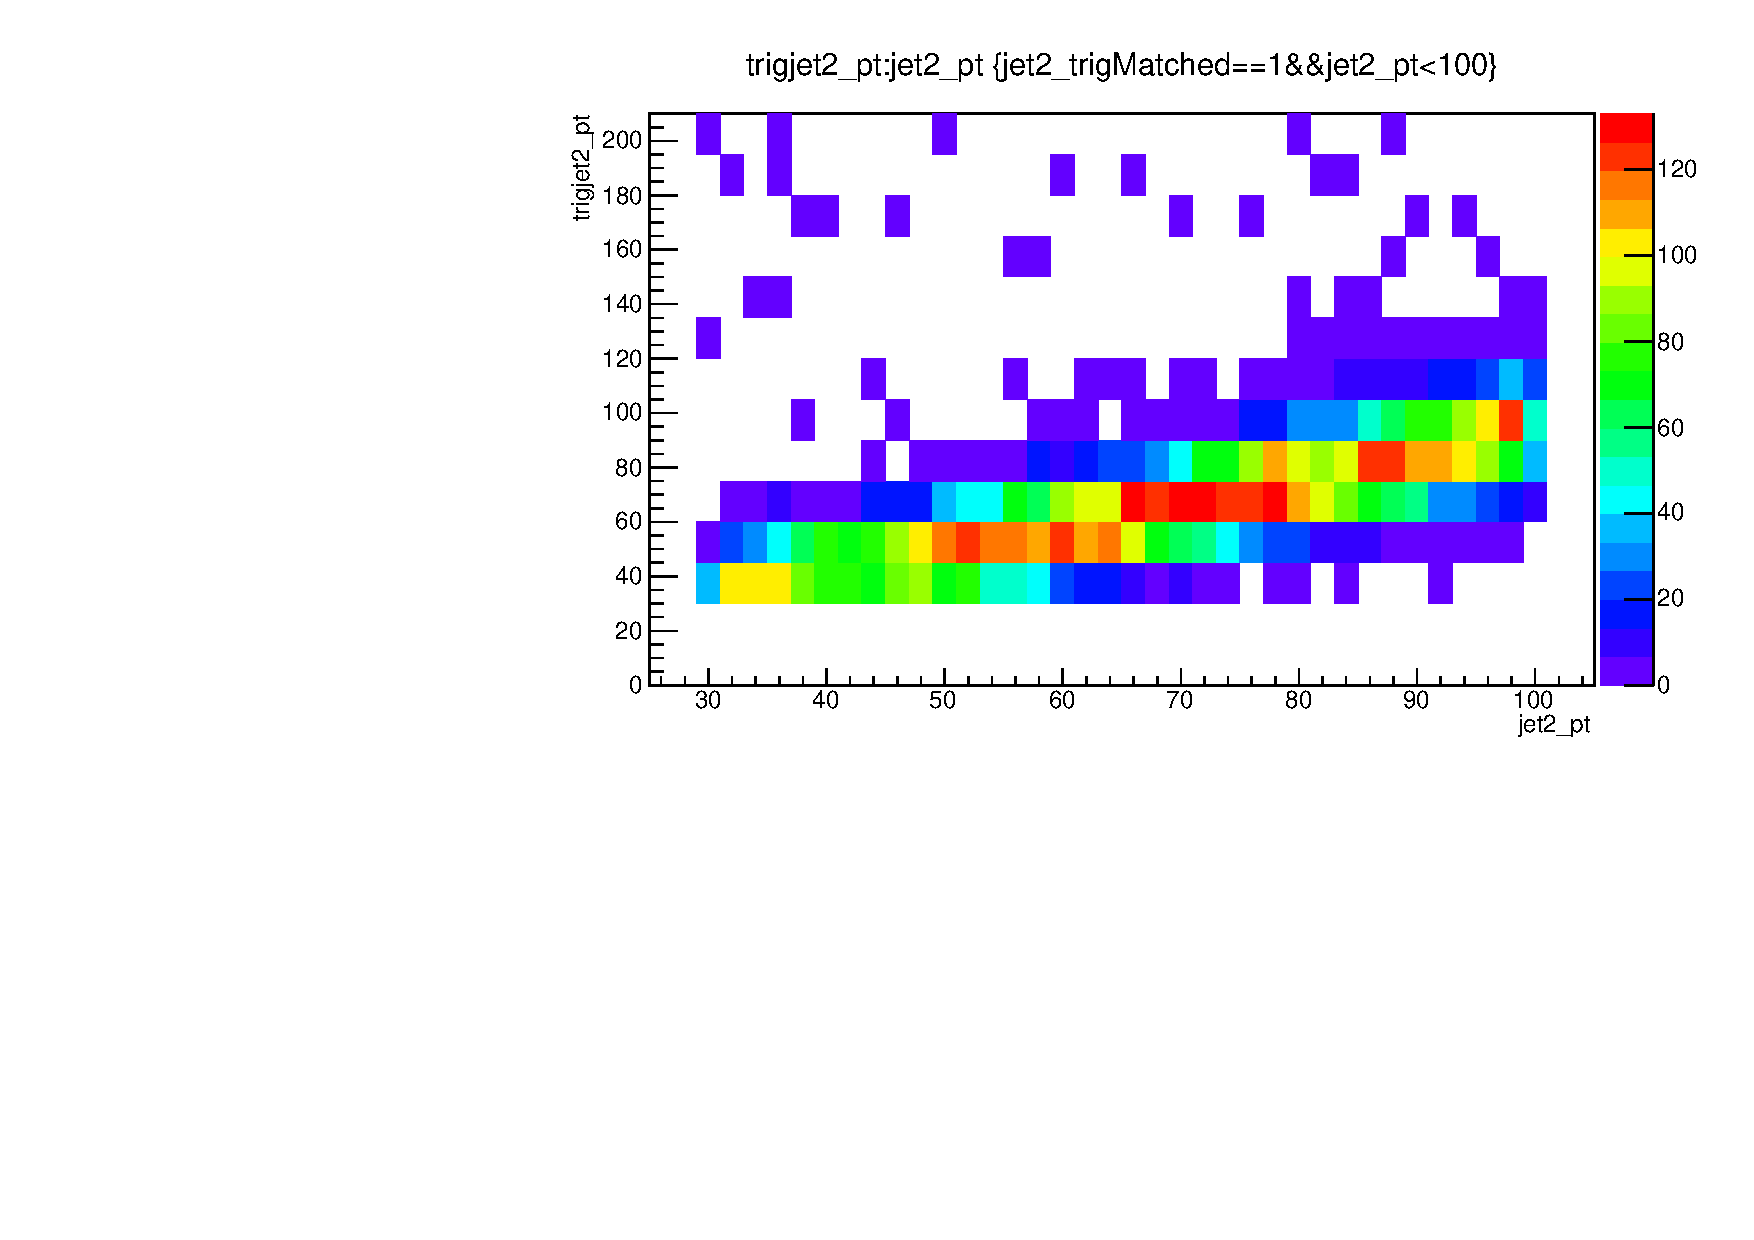
\includegraphics[width=.5\textwidth]{TalkPics/trigeff021115/trigeffstudies/jet2calotrigresponsept<100.pdf}
\end{frame}

\begin{frame}
  \frametitle{Summary}
  \label{lastframe}
  \scriptsize
  \begin{block}{}
    \begin{itemize}
    \item L1ETM60 fully efficient at $\sim$200 GeV
    \item Requiring L1ETM60 in the denominator improves trigger turn ons
    \item[-] Indicates part of the inefficiency seen is due to L1
    \item Jet $p_{T}$ still less efficient than in run 1
    \item[-] Calo jets with 30 GeV $p_{T}$ frequently have offline $p_{T}$ above pf trigger threshold
    \item[-] Could cause inefficiencies
    \item[-] Needs more investigation: We currently only have trigger jet information for events that pass the trigger
    \item[-] Reemulating trigger on raw data so we can check if events failing trigger fail calo filter or pf filter
    \end{itemize}
  \end{block}
  \centering
\end{frame}

%UPDATED BACKUP
\begin{frame}
  \frametitle{Backup}
\end{frame}

\begin{frame}
\end{frame}

\end{fmffile}
\end{document}
